\documentclass{article}

\usepackage{opts}
\usegdlibrary{trees,phylogenetics}

\begin{document}

\listoffigures
\clearpage

\tikzsetnextfilename{trump-kim-en}
\begin{figure}
  \centering\resizebox{.8\textwidth}{!}{
    \begin{tikzpicture}[%
      decoration={amplitude=1.5pt}, penciline={jag ratio=1},%
      chain/.style={on chain},%
      node distance=5mm,%
      tight/.style={outer sep=-3mm, inner sep=0pt}]

      {[start chain=1 going below,%
        every on chain/.style={join={by ->, decorate,%
            "{\purisa Ask for service}" {scale=.4, inner sep=2pt},%
          }},%
        every node/.style={inner sep=0pt,align=center, minimum height=1.3cm}]%
    
        \node (trump) [chain,label={-120,scale=.4,label distance=-9mm:{\boss}}] {\trump};%
    
        \node (trmale) [chain,label={left,scale=.4:{\cnwp}},%
        label={-105,scale=.4,label distance=-6mm:{\translator}}] {\trmale};%
    
        \node (secmale) [chain,label={-120,scale=.4,label distance=-9mm:{\secretary}}] {\secmale};
      }
  
      {[start chain=2 going below,%
        every on chain/.style={join={by <-,decorate,%
            "{\purisa Provide service}"' {scale=.4, inner sep=2pt}}},%
        every node/.style={inner sep=0pt,align=center, minimum height=1.3cm}]%

        \node (kim) [chain,right=2.5cm of trump,%
        label={-60,scale=.4,label distance=-9mm:{\boss}}] {\kim}%
        edge [decorate,dashed,<->, "{\purisa Topic}" {scale=.5, tight},%
        "\protocol"' {scale=.5, tight}] (trump);%

        \node (trfemale) [chain, label={right,scale=.4,xshift=-1em:{\cnwp}},%
        label={-60,scale=.4,label distance=-9mm:{\translator}}] {\trfemale}%
        edge [decorate,dashed,<->,"{\cnfont 中文}" {scale=.5, tight},%
        "\protocol"' {scale=.5, tight}] (trmale);%

        \node (secfemale) [chain, label={-60,scale=.4,label distance=-9mm:{\secretary}}]%
        {\secfemale} edge [decorate,dashed,<->, "{\purisa Fax}" {scale=.5, tight},%
        "\protocol"' {scale=.5, tight}] (secmale);%
      }
  
      \node [ellipse callout, callout absolute pointer={(kim.80)},%
      above right=5pt of kim, xshift=-15pt, scale=.4, draw] {\krwp};%

      \node [ellipse callout, callout absolute pointer={(trump.110)}, align=center,%
      above left=5pt of trump, xshift=10pt, scale=.4, draw] {\enwp};%

      \path [draw,->,decorate] (secmale) |- ($(secfemale.south)+(0,-3mm)$) -- (secfemale);
\end{tikzpicture}}
\caption{Layered design\label{fig:trump-kim}}
\end{figure}

\tikzsetnextfilename{hierarchy-subnet}
\begin{figure}
  \centering
  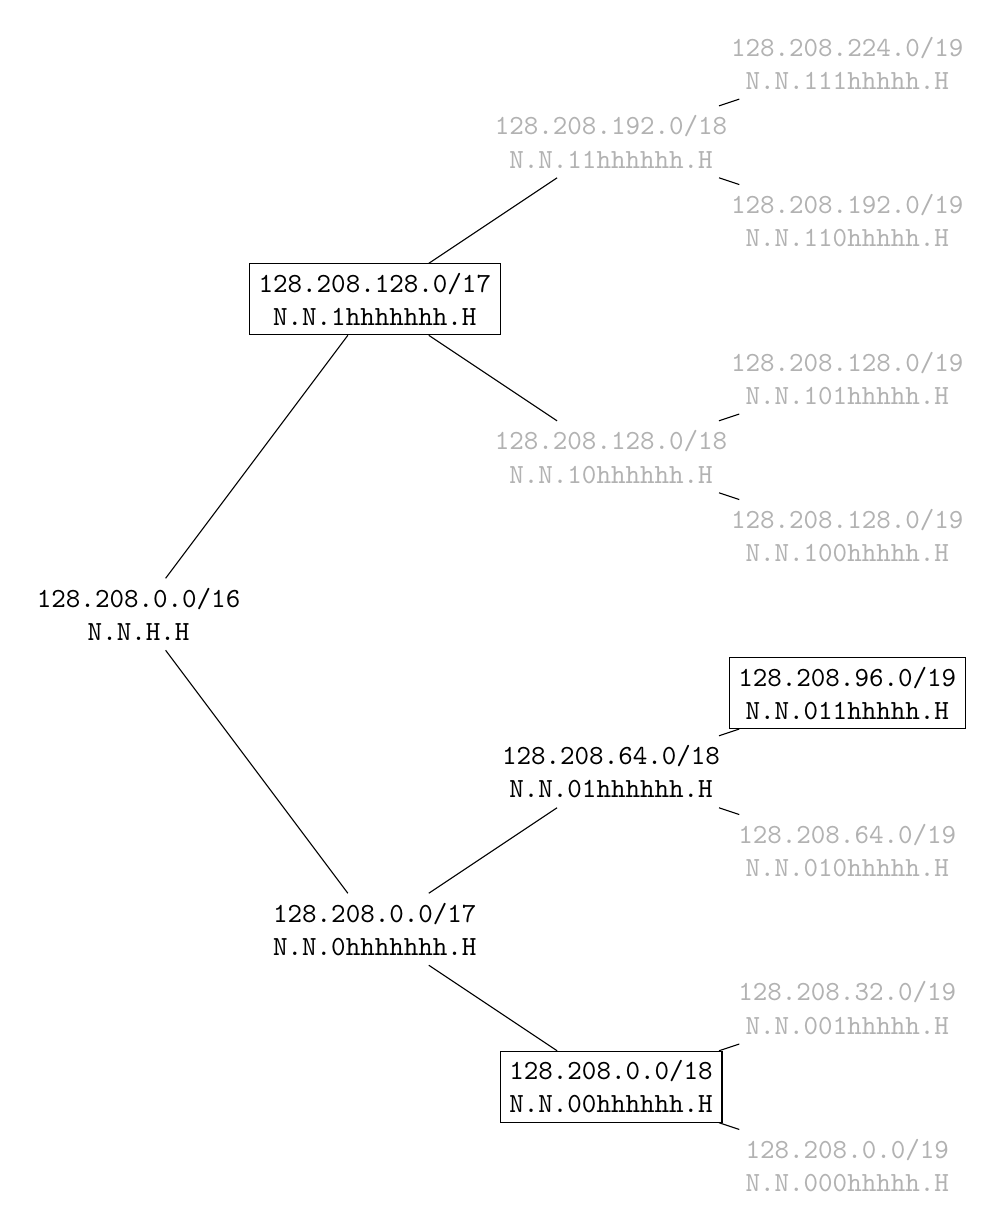
\begin{tikzpicture}[align=center,font=\ttfamily,%
  level distance=3cm,
  level 1/.style={sibling distance=8cm},%
  level 2/.style={sibling distance=4cm},
  level 3/.style={sibling distance=2cm}]
  
  \node {128.208.0.0/16\\N.N.H.H} [grow=0]
  child {node {128.208.0.0/17\\N.N.0hhhhhhh.H}
    child {node [draw] {128.208.0.0/18\\N.N.00hhhhhh.H}
      child {node [opacity=.3] {128.208.0.0/19\\N.N.000hhhhh.H}}
      child {node [opacity=.3] {128.208.32.0/19\\N.N.001hhhhh.H}}
    }
    child {node {128.208.64.0/18\\N.N.01hhhhhh.H}
      child {node [opacity=.3] {128.208.64.0/19\\N.N.010hhhhh.H}}
      child {node [draw] {128.208.96.0/19\\N.N.011hhhhh.H}}
    }
  }
  child {node [draw] {128.208.128.0/17\\N.N.1hhhhhhh.H}
    child {node [opacity=.3] {128.208.128.0/18\\N.N.10hhhhhh.H}
      child {node [opacity=.3] {128.208.128.0/19\\N.N.100hhhhh.H}}
      child {node [opacity=.3] {128.208.128.0/19\\N.N.101hhhhh.H}}
    }
    child {node [opacity=.3] {128.208.192.0/18\\N.N.11hhhhhh.H}
      child {node [opacity=.3] {128.208.192.0/19\\N.N.110hhhhh.H}}
      child {node [opacity=.3] {128.208.224.0/19\\N.N.111hhhhh.H}}
    }
  };
\end{tikzpicture}
  \caption{Subnet hierarchy}
  \label{fig:subnet}
\end{figure}

\tikzsetnextfilename{subnet-194}
\begin{figure}%\resizebox{\textwidth}{!}{
  \centering
    \begin{tikzpicture}
    \graph [phylogenetic tree layout,grow'=right, sibling distance=.5cm,
    nodes={inner sep=0pt,font=\ttfamily},
    empty nodes, edge quotes mid, length=3,
    edges={nodes={sloped,fill=white}}]%
    {
      16 [as={194.24.0.0/16},inner sep=2pt] -- {
        17a [>"194.24.0.0/17"] -- {
          18a [>"192.24.0.0/18"] -- {
            19a [>"194.24.0.0/19"] -- {
              20a [>"194.24.0.0/20"] -- {
                21a [>"194.24.0.0/21"],
                21b [>"194.24.8.0/21"] -- {22a [>"194.24.8.0/22"], 22b [>"194.24.12.0/22"]}},
              20b [>"194.24.16.0/20"]}, 19b [>"194.24.32.0/19"]},
          18b [>"194.24.64.0/18"]}, 17b [>"194.24.128.0/17"]}
    };
  \end{tikzpicture}
  \caption{Subnetting example - 194.24.0.0/16\label{fig:subnet-194}}%}
\end{figure}

\tikzsetnextfilename{State}
\begin{figure}
  \centering\resizebox{\textwidth}{!}{
    \begin{tikzpicture}
      %%% background image
      \node[anchor=south west,inner sep=0] (image) at (0.1,0.1)%
      {\includegraphics[width=\paperwidth]{state}};

      % http://tex.stackexchange.com/questions/9559/drawing-on-an-image-with-tikz
      \begin{scope}[x={(image.south east)},y={(image.north west)}]%
        % %%% grid
        % \draw[help lines,xstep=.1,ystep=.1] (0,0) grid (1,1);%
        % \foreach \x in {0,1,...,9} { \node [anchor=north] at (\x/10,0) {0.\x}; }%
        % \foreach \y in {0,1,...,9} { \node [anchor=east] at (0,\y/10) {0.\y}; }%

        \draw [dashed] (0,0) -- (0,.32) -- (.63,.32) -- (.63,0) -- cycle;%
        \node (activeclose) at (.3,-.01) {\emph{active close}};%

        \draw [dashed] (.68,0) -- (.68,.32) -- (.97,.32) -- (.97,0) -- cycle;%
        \node (passiveclose) at (.82,-.01) {\emph{passive close}};

        \node (simultaneousclose) at (.47,.31) {\emph{simultaneous close}};%
        \node (simultaneousopen) at (.46,.55) {\emph{simultaneous open}};%
        \node (established) at (.44,.36) {\emph{data transfer state}};%
        \node (passiveopen) at (.45,.79) {\emph{passive open}};
      \end{scope}
    \end{tikzpicture}}
  \caption{TCP state transition diagram}
  \label{fig:tcp-state}
\end{figure}

\tikzsetnextfilename{Apache}
\begin{figure}
  \centering\resizebox{.7\textwidth}{!}{
\begin{tikzpicture}
  \begin{pgfonlayer}{background}
    \node [inner sep=0] at (current page.center) {
      \includegraphics[width=\paperwidth]{imgs/apache}};
  \end{pgfonlayer}
  \node [shift={(5.3cm,-3cm)},scale=2.5] at (current page.center) {
    \textbf{Apache HTTP Server}};
\end{tikzpicture}  }
  \caption{Apache HTTP Server}
  \label{fig:Apache}
\end{figure}

\tikzsetnextfilename{HTTP}
\begin{figure}
  \centering\resizebox{.7\textwidth}{!}{
\begin{tikzpicture}[auto,%
  every node/.style = {inner sep=0pt},%
  every edge/.style = {blue!50,ultra thick,bend left,draw,->},%
  every edge quotes/.style = {blue!50,sloped,align=center,inner sep=1pt},%
  help lines/.style={very thin,dotted},%
  xy/.style={font=\dejavu\tiny},inner sep=1pt]
  
  %%% background image
  \node (apache) [anchor=south west,%
  label={below,shift={(1cm,1mm)},scale=.5:{\purisa Apache HTTP Server}}] %
  at (0,0) {\includegraphics[width=5cm]{imgs/apache}}; %

  \node (chrome) [left=2cm of apache.south west, anchor=south east]%
  {
\includegraphics[width=1cm]{imgs/gchrome}}%
  edge ["HTTP Request\\{\small (URL + Verb)}" scale=.7] ($(apache.center)+(-1.5cm,0)$);

  \path (apache) edge ["HTTP Response\\{\small (Status code + Message body)}" %
  {scale=.7,shift={(2cm,0)}}] (chrome);%

\end{tikzpicture}  }
  \caption{HTTP client/server interaction}
  \label{fig:HTTP}
\end{figure}

\tikzsetnextfilename{Chains}
\begin{figure}
  \centering\resizebox{.6\textwidth}{!}{
\begin{tikzpicture}[
  every node/.style ={inner sep=2pt, rounded corners,},
  every edge/.style ={draw,black!50, ->, thick},
  chain/.style ={fill=red!50, circle, minimum size=50pt, scale=.7},
  pin distance=7pt, pin edge={->,thick,solid},
  ]
  
  \node [chain] (forward) at (current page.center) {FORWARD};
  \node [left=.7cm of forward, scale=.7, align=center, fill=blue!50] (routing) {Routing\\Decision};
  \node [chain, below=.7cm of routing, pin={below:{\tiny Local Process}}] (input) {INPUT};
  \node [chain, right=1.7cm of input, pin={[pin edge={<-,thick,solid}]below:{\tiny Local Process}}] (output) {OUTPUT};
  \node [left=of routing, label={above right:{\tiny Incoming}}] (in) {};
  \node [right=1.5cm of forward, label={above left:{\tiny Outgoing}}] (out) {};
  
  \path (in) edge (routing) (routing) edge (forward) edge (input) (forward) edge (out);
  \draw[black!50,->,thick] (output) -- ($(forward)!(output)!(out)$);
\end{tikzpicture}}
  \caption{iptables chains}
  \label{fig:Chains}
\end{figure}

\tikzsetnextfilename{dns-nonrecur}
\begin{figure}
  \centering\resizebox{.8\textwidth}{!}{
\begin{tikzpicture}[auto,node distance=15pt,%
  server node/.style ={inner sep=2pt, rounded corners, fill=red!30,align=center,font=\dejavu},%
  chrome/.style = {circle,inner sep=0pt},%
  every edge/.style ={draw,black!50, ->, thick},%
  every edge quotes/.style = {sloped,scale=.5,font=\small,font=\ttfamily},%
  red edge/.style = {bend left=10, red!70},%
  violet edge/.style = {bend left=10, violet!70},%
   ]%
  
   \node (local) [server node,circle,align=center, scale=.6]%
   {Local\\DNS server\\(dns.swfu.edu.cn)};%
  
  \node (chrome1)       [left=of local,chrome] {
\includegraphics[width=15pt]{gchrome}};%
  \node (chrome2) [above left=of local,chrome] {
\includegraphics[width=15pt]{gchrome}};%
  \node (chrome3) [below left=of local,chrome] {
\includegraphics[width=15pt]{gchrome}};%

  \node [server node, right=100pt of local] (almond) {almond.nuts.com};
  \node [server node, above=of almond.north west,anchor=south west] (root)%
  {Root DNS server\\[-3pt](dns.edu.cn)};%
  \node [server node, below=of almond.south west,anchor=north west] (pack)%
  {pack.plant.nuts.com};%

  \path
  (local.5)    edge ["sale.plant.nuts.com",violet!70] (almond.176)%
  (almond.184) edge ["plant.nuts.com NS pack.plant.nuts.com", orange] (local.354)%

  (local.60) edge ["sale.plant.nuts.com",bend left=5, violet!70] (root.177)%
  (root.182) edge ["nuts.com NS almond.nuts.com" {near end,rotate=-4},bend right=5, blue!70] (local.45)%

  (local.320) edge ["sale.plant.nuts.com" {near start,rotate=3},bend right=5, violet!70] (pack.177)%
  (pack.184)  edge ["sale.plant.nuts.com A 172.16.6.4" {near start,xshift=-4em,rotate=-2},bend left=5, Green] (local.305)%

  (chrome1) edge [red edge] (local)%
  (chrome2) edge [red edge] (local)%
  (chrome3) edge [red edge] (local)%
  (local)   edge [violet edge] (chrome1)%
  (local)   edge [violet edge] (chrome2)%
  (local)   edge [violet edge] (chrome3);%
\end{tikzpicture}  }
  \caption{DNS non-recursive transaction}
  \label{fig:dns-nonrecur}
\end{figure}

\tikzsetnextfilename{dns-sw}
\begin{figure}
  \centering\resizebox{.6\textwidth}{!}{
\begin{tikzpicture}[auto,%
  every node/.style ={inner sep=2pt, color=black!60},%
  server/.style = {circle,align=center,fill=gray!10,rounded corners},%
  every edge/.style ={draw,->,bend left,black!50,thick},%
  every edge quotes/.style = {black!50,scale=.4,sloped}%
  ]%
  
  \node [server,scale=.5] (resolver) {DNS\\resolver};%
  \node [server] (server) [right=of resolver] {DNS\\server};%
  \path
  (resolver) edge ["DNS query" xshift=3em] (server)%
  (server)   edge ["DNS response" xshift=3em] (resolver);
\end{tikzpicture}  }
  \caption{DNS overview}
  \label{fig:dns-sw}
\end{figure}

\tikzsetnextfilename{http-Req}
\begin{figure}
  \centering\resizebox{\textwidth}{!}{
\begin{tikzpicture}[auto,%
  every edge/.style ={red!50,thick,draw,->},%
  every node/.style ={red!50,rounded corners,inner sep=2pt}%
  ]%
  
  %%% background image
  \node[anchor=south west,inner sep=0] (image) at (0,0)%
  {\includegraphics[width=\paperwidth]{http-req}};

  % http://tex.stackexchange.com/questions/9559/drawing-on-an-image-with-tikz
  \begin{scope}[x={(image.south east)},y={(image.north west)}]%
    % %%% grid
    % \draw[help lines,xstep=.1,ystep=.1] (0,0) grid (1,1);%
    % \foreach \x in {0,1,...,9} { \node [anchor=north] at (\x/10,0) {0.\x}; }%
    % \foreach \y in {0,1,...,9} { \node [anchor=east] at (0,\y/10) {0.\y}; }%

    \node (req) at (.57,.65) {Request line};%
    \node (header) [below=.32 of req.west,anchor=west]{Header lines};%
    \node (bracket) [inner sep=0,left=of header] {$ \left\} \rule{0pt}{13mm}\right. $};%
    \node (blank) [below=.3 of header.west,anchor=west] {Empty line};%
  \path%
  (req.west) edge ++(-.05,0)%
  (blank.west) edge  ++(-.47,0)%
  (header.west) edge (bracket.east);
  \end{scope}
\end{tikzpicture}  }
  \caption{HTTP request}
  \label{fig:http-Req}
\end{figure}

\tikzsetnextfilename{http-Res}
\begin{figure}
  \centering\resizebox{.7\textwidth}{!}{
\begin{tikzpicture}[auto,node distance=5pt,%
  every edge/.style ={red!50,thick,draw,->},%
  every node/.style ={red!50,rounded corners,inner sep=2pt,font=\LARGE}%
  ]%

  %%% background image
  \node[anchor=south west,inner sep=0] (image) at (0,0)%
  {\includegraphics[width=\paperwidth]{http-res}};

  % http://tex.stackexchange.com/questions/9559/drawing-on-an-image-with-tikz
  \begin{scope}[x={(image.south east)},y={(image.north west)}]%
    % %%% grid
    % \draw[help lines,xstep=.1,ystep=.1] (0,0) grid (1,1);%
    % \foreach \x in {0,1,...,9} { \node [anchor=north] at (\x/10,0) {0.\x}; }%
    % \foreach \y in {0,1,...,9} { \node [anchor=east] at (0,\y/10) {0.\y}; }%

  \node (status) at (.85,.975) {Status line};%
  \node (header) [below=.24 of status.west,anchor=west]{Header lines};%
  \node (bracket) [left=of header,inner sep=0]%
  {$ \left\} \rule{0pt}{38mm}\right. $};%
  \node (blank) [below=.24 of header.west,anchor=west]{Empty line};%
  \node (data) [below=.25 of blank.west,anchor=west,xshift=-4cm]{Data};%
  \node (bracket2) [left=of data,inner sep=0] {$ \left\} \rule{0pt}{38mm}\right. $};%
  \path%
  (status.west) edge ++(-.43,0)%
  (blank.west)  edge ++(-.7,0);%
  \end{scope}
\end{tikzpicture}  }
  \caption{HTTP Response}
  \label{fig:http-Res}
\end{figure}

\tikzsetnextfilename{http-transaction}
\begin{figure}
  \centering\resizebox{\textwidth}{!}{
\begin{tikzpicture}[auto,node distance=0pt,%
  every node/.style ={inner sep=0},%
  every edge/.style ={draw,->,thick},%
  every edge quotes/.style = {scale=.4,sloped,inner sep=1pt,font=\ttfamily},%
  server/.style = {rounded corners, fill=black!30, inner sep=2pt},%
  ]%
  
  \node (dns) [color=violet!70, label={[violet!70]below:{\scriptsize DNS Lookup}}]%
  {\rule{23mm}{4pt}};

  \node (connect) [right=of dns,color=orange, label={[orange]below:{\scriptsize Connect}}]%
  {\rule{20mm}{4pt}};

  \node (send) [right=of connect,color=Green, label={[Green]below:{\scriptsize Send}}]%
  {\rule{6mm}{4pt}};

  \node (wait) [right=of send,color=red!70, label={[red!70]below:{\scriptsize Wait}}]%
  {\rule{12mm}{4pt}};

  \node (load) [right=of wait,color=blue!50, label={[blue!50]below:{\scriptsize Load}}]%
  {\rule{20mm}{4pt}};

  \node (dnsserver) [above=2cm of dns.west,anchor=west,server] {DNS Server};%
  \node (webserver) [right=of dnsserver.east,anchor=west,server,minimum width=60mm] {Web Server};%

  % \node [above=of dnsserver, xshift=4.2cm, yshift=5mm] {\underline{Simple HTTP Transaction}};

  \path%
  (dns.north west) edge ["DNS query" near end,violet] (dnsserver.200)%
  (dnsserver.340)  edge ["IP address" near start,violet] (dns.north east)%
  (connect.north west) edge ["SYN",orange] (webserver.185)%
  (webserver.185) edge ["SYN/ACK" near start,orange] (connect.north)%
  (connect.north) edge ["ACK",orange] (webserver.190)%
  (send.north west) edge ["HTTP request" near end] (webserver.220)%
  (webserver.250) edge ["HTTP response"' near end,"1\textsuperscript{st} segment" near start,red!70]%
  (wait.north east)%
  (webserver.335) edge ["PSH"',"2\textsuperscript{nd} segment" near start,blue!50] (load.170)%
  (load.145) edge ["ACK" near end,blue!50] (webserver.354)%
  (webserver.349) edge ["HTTP\_Continue"' near end,"3\textsuperscript{rd} segment" near start,blue!50] (load.20)%
  (webserver.355) edge ["FIN",black!60] (load.north east);%
\end{tikzpicture}  }
  \caption{HTTP transaction}
  \label{fig:http-transaction}
\end{figure}

\tikzsetnextfilename{persistent-transaction}
\begin{figure}
  \centering\resizebox{\textwidth}{!}{
\begin{tikzpicture}[auto,node distance=0pt,%
  every node/.style ={inner sep=0},%
  every edge/.style ={draw,->,thick},%
  every edge quotes/.style = {scale=.5,sloped,inner sep=1pt,font=\ttfamily},%
  server/.style = {rounded corners, fill=black!30, inner sep=2pt},%
  ]%
  
  \node [color=violet!70, label={[violet!70]below:{\scriptsize DNS Lookup}}]
  (dns) {\rule{25mm}{4pt}};

  \node [color=orange, label={[orange]below:{\scriptsize Connect}},
  right=of dns] (connect) {\rule{20mm}{4pt}};

  \node [color=Green, label={[Green]below:{\scriptsize Send}},
  right=of connect] (send) {\rule{7mm}{4pt}};

  \node [color=red!70, label={[red!70]below:{\scriptsize Wait}},
  right=of send] (wait) {\rule{18mm}{4pt}};

  \node [color=blue!50, label={[blue!50]below:{\scriptsize Load}},
  right=of wait] (load) {\rule{6mm}{4pt}};

  \node [color=Green, label={[Green]below:{\scriptsize Send}},
  right=of load] (send2) {\rule{7mm}{4pt}};

  \node [color=red!70, label={[red!70]below:{\scriptsize Wait}},
  right=of send2] (wait2) {\rule{18mm}{4pt}};

  \node [color=blue!50, label={[blue!50]below:{\scriptsize Load}},
  right=of wait2] (load2) {\rule{6mm}{4pt}};
  
  \node (dnsserver) [above=2cm of dns.west,anchor=west,server,minimum width=25mm] {DNS Server};%
  \node (webserver) [right=of dnsserver.east,anchor=west,server,minimum width=83mm] {Web Server};%

  \node [below=5mm of dns.west,anchor=west,server, minimum width=77mm] (r1) {{\tiny Request I}};%
  \node [right=of r1,server,minimum width=31mm] (r2) {{\tiny Request II}};%
  
  % \node [above=of dnsserver, xshift=4.2cm, yshift=5mm] {\underline{Persistent HTTP Transaction}};

  \path%
  (dns.north west) edge ["DNS query" near end,violet] (dnsserver.200)%
  (dnsserver.340)  edge ["IP address" near start,violet] (dns.north east)%
  (connect.north west) edge ["SYN",orange] (webserver.184)%
  (webserver.184) edge ["SYN/ACK" near start,orange] (connect.7)%
  (connect.7) edge ["ACK",orange] (webserver.186)%
  (send.north west) edge ["HTTP request" near end,Green] (webserver.190)%
  (webserver.195) edge ["HTTP response" near start,red!70] (wait.north east)%
  (send2.north west) edge [Green] (webserver.353)%
  (webserver.355) edge [red!70] (wait2.north east);%
\end{tikzpicture}  }
  \caption{HTTP persistent transaction}
  \label{fig:persistent-transaction}
\end{figure}

\tikzsetnextfilename{resolver}
\begin{figure}
  \centering\resizebox{.6\textwidth}{!}{
\begin{tikzpicture}[auto,%  
  every node/.style ={inner sep=2pt, rounded corners},%
  every edge/.style ={draw,black!50, ->, thick},%
  every edge quotes/.style = {font=\ttfamily,scale=.25,inner sep=2pt,align=center},%
  protocol/.style = {color=black!60,fill=gray!50},%
  pin distance=7pt, pin edge={->,thick},%
  ]  

  \node (ssh) [protocol] {SSH};%
  \node (tcp) [protocol,below=15pt of ssh, pin={[inner sep=0pt]below:{}}] {TCP};%
  
  \node (resolver) [left=20pt of ssh,fill=red!40] {{\tiny resolver}};%
  \node (cs3) [above=10pt of ssh, color=black!50, scale=.6,font=\purisa] {{\tiny cs3.swfu.edu.cn}};%

  \path%
  (cs3) edge (ssh)%
  (ssh) edge ["establish\\connection\\with IP address"] (tcp)%
  (ssh) edge [bend right,red!50,"cs3.swfu.edu.cn"' xshift=4em,] (resolver.north east)%
  (resolver.south east) edge [bend right,red!50,"202.203.132.245"' xshift=4em,] (ssh);
\end{tikzpicture}  }
  \caption{DNS resolver}
  \label{fig:resolver}
\end{figure}

\tikzsetnextfilename{tcp-socket}
\begin{figure}
  \centering\resizebox{\textwidth}{!}{
\begin{tikzpicture}[auto,node distance=0pt,inner sep=0pt,%
  note/.style = {color=black!50},%
  socket/.style = {color=blue!50!black},%
  connection/.style = {color=violet!80},%  
  every pin/.style = {pin distance=1mm, inner sep=2pt, pin edge={black!50,thick,draw}},%
  ]
  
  %%% background image
  \node[anchor=south west,inner sep=0] (image) at (0,0)%
  {\includegraphics[width=\paperwidth]{tcp-connection}};

  % http://tex.stackexchange.com/questions/9559/drawing-on-an-image-with-tikz
  \begin{scope}[x={(image.south east)},y={(image.north west)}]%
    % %%% grid
    % \draw[help lines,xstep=.1,ystep=.1] (0,0) grid (1,1);%
    % \foreach \x in {0,1,...,9} { \node [anchor=north] at (\x/10,0) {0.\x}; }%
    % \foreach \y in {0,1,...,9} { \node [anchor=east] at (0,\y/10) {0.\y}; }%

    \node (local) [note, pin={[note]below:{address}}] at (.267,0)%
    {\rule{14em}{1.2pt}};
    
    \node (lport) [note, pin={[note]below:{port}},right=.8em of local]%
    {\rule{3.7em}{1.2pt}};

    \node (remote) [note, pin={[note]below:{address}},right=3em of lport]%
    {\rule{11.1em}{1.2pt}};

    \node [note, pin={[note]below:{port}},right=1em of remote]%
    (rport) {\rule{4.5em}{1.2pt}};

    \node [socket, pin={[socket,pin edge={blue!50,thick}]below:{socket}},%
    below=4ex of local.west,anchor=west] (lsocket) {\rule{18.5em}{2pt}};
    
    \node [socket, pin={[socket,pin edge={blue!50,thick}]below:{socket}},%
    below=4ex of remote.west,anchor=west] (rsocket) {\rule{16.6em}{2pt}};
    
    \node (connection) [connection, below=4ex of lsocket.west,anchor=west,%
    pin={[connection,pin edge={violet!50,thick}]below:{%
        a pair of sockets form a TCP connection}}] {\rule{38.2em}{2pt}};
  \end{scope}
\end{tikzpicture}  }
  \caption{TCP socket pair}
  \label{fig:tcp-socket}
\end{figure}

\tikzsetnextfilename{Url}
\begin{figure}
  \centering\resizebox{\textwidth}{!}{
\begin{tikzpicture}[auto,inner sep=0pt,%
  note/.style = {blue},%
  every pin/.style = {blue,pin distance=2pt,pin edge={blue!50,thick,draw},inner sep=2pt},%
  ]%
  
  %%% background image
  \node[anchor=south west,inner sep=0] (image) at (0,0)%
  {\includegraphics[width=\paperwidth]{url}};

  % http://tex.stackexchange.com/questions/9559/drawing-on-an-image-with-tikz
  \begin{scope}[x={(image.south east)},y={(image.north west)}]%
    % %%% grid
    % \draw[help lines,xstep=.1,ystep=.1] (0,0) grid (1,1);%
    % \foreach \x in {0,1,...,9} { \node [anchor=north] at (\x/10,0) {0.\x}; }%
    % \foreach \y in {0,1,...,9} { \node [anchor=east] at (0,\y/10) {0.\y}; }%

    \node (protocol) [note,pin={below:{protocol}}] at (0,-.2) [anchor=west] {\rule{4em}{2pt}};%
    
    \node (host) [note,pin={above:{host}}] at (.115,1.2) [anchor=west] {\rule{15.3em}{2pt}};%
    
    \node (resource) [note,pin={below:{resource path}}] at (.38,-.2) [anchor=west]%
    {\rule{10.8em}{2pt}};% 

    \node (query) [note,pin={above:{query}}] at (.56,1.2) [anchor=west] {\rule{27em}{2pt}};
  \end{scope}
\end{tikzpicture}  }
  \caption{URL}
  \label{fig:Url}
\end{figure}

\tikzsetnextfilename{hdrs}
\begin{figure}
  \centering\resizebox{\textwidth}{!}{
    \begin{tikzpicture}[auto,%
      node distance=0pt,inner sep=0pt,%
      minimum height=1cm,minimum width=1cm,align=center,%
      kept/.style = {fill=yellow!90!red},%
      gone/.style = {fill=red!30},%
      change/.style= {fill=blue!30},%
      new/.style= {fill=green!30}
  ]%
  \node (ver4) [kept,text width=1cm,font=\small] {Version};%
  \node (ihl) [right=of ver4,gone] {IHL};%
  \node (tos) [right=of ihl,change,text width=2cm] {Type of\\Service};%
  \node (tot) [right=of tos,change,text width=4cm]{Total Length};%
  \node (id)  [below=of ver4.south west, anchor=north west,gone,text width=4.025cm]
  {Identification};%
  \node (flag) [right=of id,gone,text width=1.67cm] {Flags};%
  \node (frag) [right=of flag,gone,text width=2.32cm] {Fragment\\Offset};%
  \node (ttl) [below=of id.south west, anchor=north west,change,text width=2cm] {Time to
    Live};%
  \node (p) [right=of ttl,change,text width=2.01cm] {Protocol};%
  \node (sum) [right=of p,gone,text width=4cm] {Header Checksum};%
  \node (src) [below=of ttl.south west,anchor=north west,kept,text width=8.04cm] {Source
    Address};%
  \node (dst) [below=of src,kept,text width=8.04cm] {Destination Address};%
  \node (opt) [below=of dst.south west, anchor=north west,gone, text width=5.5cm] {Options};%
  \node (pad) [right=of opt,gone, text width=2.53cm]{Padding};%

  \node (ver6) [right=1cm of tot,kept,text width=1cm,font=\small] {Version};%
  \node (tc) [right=of ver6,change,text width=2cm] {Traffic Class};%
  \node (fl) [right=of tc,new,text width=5cm] {Flow Label};%
  \node (pl) [below=of ver6.south west, anchor=north west,change, text width=4cm] {Payload
    Length};%
  \node (next) [right=of pl,change,text width=2cm] {Next Header};%
  \node (hop) [right=of next,change,text width=2cm] {Hop Limit};%
  \node (src6) [below=of pl.south west, anchor=north west,kept,minimum width=8.03cm, minimum
  height=4cm] {Source Address};%
  \node (dst6) [below=of src6,kept,minimum width=8.03cm, minimum height=4cm] {Destination
    Address};%

  \node (kept) [below=1cm of opt,xshift=-2cm,kept,minimum size=3mm,%
  label={right,align=left,inner sep=3pt:{kept field}}] {};%
  \node (gone) [below=2mm of kept,gone,minimum size=3mm, label={right,align=left,inner sep=3pt:{gone
      field}}] {};%
  \node (change) [below=2mm of gone,change,minimum size=3mm,
  label={right,align=left,inner sep=3pt:{changed field}}] {};%
  \node (new) [below=2mm of change,new,minimum size=3mm, label={right,align=left,inner sep=3pt:{new
      field}}] {};%
  % \node (link) [below=5mm of new,font=\tiny\ttfamily] {\url{https://www.cisco.com/en/US/technologies/tk648/tk872/technologies_white_paper0900aecd8054d37d.html}};

  \node [above left=of tot,xshift=1cm]{IPv4 Header};
  \node [above right=of tc]{IPv6 Header};
  
\end{tikzpicture}  }
  \caption{IPv4 header vs. IPv6 header}
  \label{fig:hdrs}
\end{figure}

\end{document}
%%% Local Variables:
%%% mode: latex
%%% TeX-master: t
%%% End:
